\documentclass[xcolor=dvipsnames]{beamer}

%%% Packages %%%
\usepackage{graphicx}
\usepackage[utf8]{inputenc}
\usepackage{subfig}
\usepackage{tikz}
\usepackage[absolute, overlay]{textpos}
\usepackage{soul}
\usepackage{booktabs}
\usepackage{multicol}
\usepackage{multimedia} % For movies
\usepackage{pgfplots} % For generating random numbers for tikz 
\usepackage{pstricks-add}
\usepackage{comment}
\usepackage{multimedia}

\usetikzlibrary{calc}
\usetikzlibrary{shapes.geometric}
\usetikzlibrary{arrows}

%%% Creating Tarleton Purple %%%
\definecolor{TarletonPurple}{RGB}{79, 45, 127}
\definecolor{ufsdxf}{rgb}{0.30980392156862746,0.17647058823529413,0.4980392156862745}


%%% Beamer Theme %%%
\usetheme{Copenhagen}
\usecolortheme[named=TarletonPurple]{structure}


%%% Graphics Path %%%
\graphicspath{{./images}}

%%% Title Page Info %%%
\title{SYNC or Swim}
\subtitle{A Particle Model of the Interaction within Fish Schools}
\author{David Ebert and Mikaela Jordan}
\institute{Tarleton State University}
\date{May $4^{th}$, 2017}

%%% Making Reference Environment For Tarleton Picture %%%
\newenvironment{reference}[2]{
\begin{textblock*}{\textwidth}(#1,#2)              
  \footnotesize\it\bgroup\color{red!50!black}}{\egroup\end{textblock*}}

%%% Setting node styles for isosceles triangles %%%
\tikzset{
	focal/.style={
		draw=Magenta,
		shape=isosceles triangle,
		fill=Magenta!30,
		shape border uses incircle,
		minimum height= 0.15cm, 
		minimum width= 0.1cm,
		shape border rotate=#1,
		isosceles triangle stretches,
		inner sep=0pt
	},
	focalfish/.style={focal=+90}
}

\tikzset{
	fish/.style={
		draw=MidnightBlue,
		shape=isosceles triangle,
		fill=MidnightBlue!50,
		minimum height= 0.15cm, 
		minimum width= 0.1cm,
		shape border rotate=90,
		isosceles triangle stretches,
		inner sep=0pt
	}
}

%%% The document %%%
\begin{document}
\makeatletter
\def\beamer@framenotesbegin{
\begin{reference}{107mm}{0.5mm}
\tikz\node[opacity=1.0]{\includegraphics[scale=0.4]{images/tsumath_copy}};
\end{reference} 
}

\frame{\titlepage}

\begin{frame}
	\frametitle{Motivation}
%	\movie{}{images/fishSwarmYT.mp4}
\end{frame}

\begin{frame}
	\frametitle{Schooling Model}
	\begin{multicols}{2}
	\onslide<1->{
	Our model represents each fish adhering to the following three rules:}
	\begin{itemize}
		\onslide<2->{
			\item \textbf{\textcolor{OliveGreen}{Alignment}}}
		\onslide<3->{
			\item \textbf{\textcolor{Maroon}{Cohesion}}}
		\onslide<4->{
			\item \textbf{\textcolor{TarletonPurple}{Separation}}}
%		Avoid collisions with neighbors
	\end{itemize}
	\begin{figure}
		\centering
		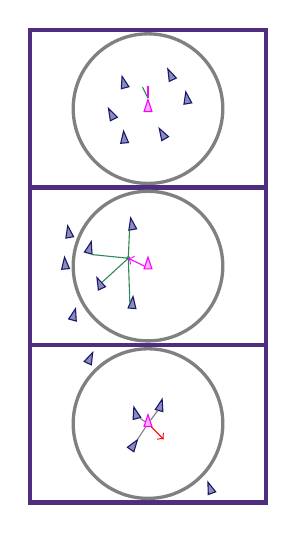
\begin{tikzpicture}
			\onslide<2>{
				\draw[ultra thick, TarletonPurple] (0, 4) rectangle (3, 6);
				\draw[very thick, gray] (1.5, 5) circle [radius=0.95cm];
				%%% Alignment %%%
				
				\node[focalfish] (focal1) at (1.5, 5) {};
				\node[fish, rotate=15] (align1) at ($(focal1) + (-0.3, 0.3)$) {};
				\node[fish, rotate=25] (align2) at ($(focal1) + (0.3, 0.4)$) {};
				\node[fish, rotate=10] (align3) at ($(focal1) + (0.5, 0.1)$) {};
				\node[fish, rotate=30] (align4) at ($(focal1) + (0.2, -0.35)$) {};
				\node[fish, rotate=5] (align5) at ($(focal1) + (-0.3, -0.4)$) {};
				\node[fish, rotate=27] (align6) at ($(focal1) + (-0.45, -0.1)$) {};
				
				\draw[Magenta] (focal1.north) -- ($(focal1.north) + (0, 0.15)$);
				\draw[SeaGreen] (focal1.north) -- ($(focal1.north) + (-0.07, 0.14)$);
			}
			
			\onslide<3>{
				\draw[ultra thick, TarletonPurple] (0, 2) rectangle (3, 4);
				\draw[very thick, gray] (1.5, 3) circle [radius=0.95cm];
				%%% Cohesion %%%
				\node[focalfish] (focal2) at (1.5, 3) {};
				\node[fish, rotate=10] (coh1) at ($(focal2) + (-0.2, 0.5)$) {};
				\node[fish, rotate=-15] (coh2) at ($(focal2) + (-0.75, 0.2)$) {};
				\node[fish, rotate=25] (coh3) at ($(focal2) + (-0.6, -0.25)$) {};
				\node[fish, rotate=-5] (coh4) at ($(focal2) + (-0.2, -0.5)$) {};
				\node[fish, rotate=10] (coh5) at ($(focal2) + (-1, 0.4)$) {};
				\node[fish, rotate=5] (coh6) at ($(focal2) + (-1.05, 0)$) {};
				\node[fish, rotate=-15] (coh7) at ($(focal2) + (-0.95, -0.65)$) {};
				
				\draw[SeaGreen] (coh1.south west) -- (1.25, 3.1);
				\draw[SeaGreen] (coh2.south east) -- (1.25, 3.1);
				\draw[SeaGreen] (coh3.north east) -- (1.25, 3.1);
				\draw[SeaGreen] (coh4.north west) -- (1.25, 3.1);
				
				\fill[SeaGreen] (1.25, 3.1) circle [radius=0.75pt];
				
				\draw[Magenta, ->] (focal2.west) -- (1.25, 3.1);
				}
				
			\onslide<4>{
				\draw[ultra thick, TarletonPurple] (0, 0) rectangle (3, 2);
				\draw[very thick, gray] (1.5, 1) circle [radius=0.95cm];
				%%% Separation %%%
				\node[focalfish] (focal) at (1.5, 1) {};
				\node[fish, rotate=15] (fish1) at ($(focal) + (-0.15, 0.1)$)  {};
				\node[fish, rotate=-15] (fish2) at ($(focal) + (0.15, 0.2)$) {};
				\node[fish, rotate=-35] (fish3) at ($(focal) + (-0.2, -0.3)$) {};
				\node[fish, rotate=20] (fish4) at ($(focal) + (0.8, -0.85)$) {};
				\node[fish, rotate=-25] (fish5) at ($(focal) + (-0.75, 0.8)$) {};
			
				\draw[thin, gray] (focal) -- (fish1);
				\draw[thin, gray] (focal) -- (fish2);
				\draw[thin, gray] (focal) -- (fish3);
			
				\draw[red, ->] (focal) -- ($(focal) + (0.2, -0.2)$);}
			
		
		\end{tikzpicture}
	\end{figure}
	\end{multicols}

\end{frame}

\begin{frame}
	\frametitle{General Mathematics}
	\begin{itemize}
		\onslide<1>{
		\item Lagrangian Algorithm}
		\onslide<2->{
		\item Metric distance model}
	\end{itemize}
	\begin{figure}
		\centering
		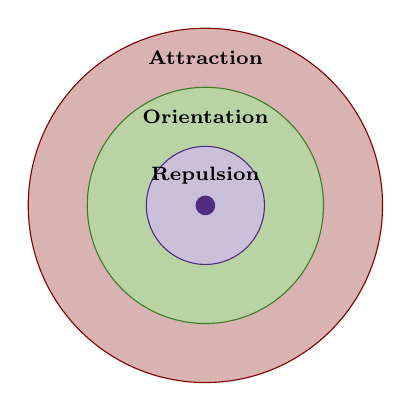
\begin{tikzpicture}[scale=0.5]
			\onslide<5->{
			\filldraw[fill=Maroon!30, draw=Maroon] (0, 0) circle [radius=4.5cm];}
			\onslide<4->{
			\filldraw[fill=OliveGreen!30, draw=OliveGreen] (0, 0) circle [radius=3cm];}
			\onslide<3->{
			\filldraw[fill=TarletonPurple!30, draw=TarletonPurple] (0, 0) circle [radius=1.5cm];}
			\onslide<3->{
			\fill[TarletonPurple] (0, 0) circle [radius=0.25cm];}
			
			\onslide<5->{
			\node at (0, 3.75) {\scriptsize{\textbf{Attraction}}};}
			\onslide<4->{
			\node at (0, 2.25) {\scriptsize{\textbf{Orientation}}};}
			\onslide<3->{
			\node at (0, 0.75) {\scriptsize{\textbf{Repulsion}}};}
		\end{tikzpicture}
	\end{figure}

\end{frame}

\begin{frame}
	\frametitle{Directional Alignment of Fish}	
		\begin{multicols}{2}
	\begin{figure}
		\centering
		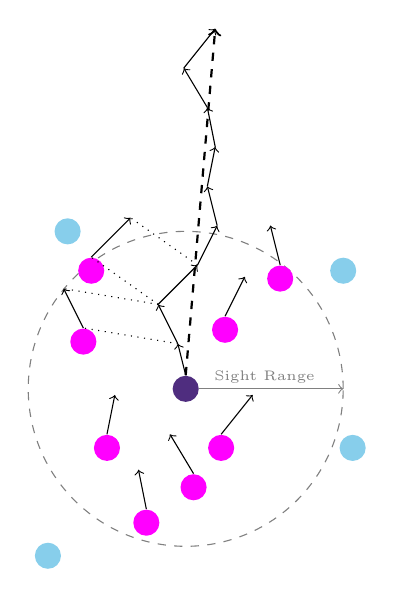
\begin{tikzpicture}[focalfish/.style={circle, minimum size=1mm, fill=TarletonPurple}, fish/.style={circle, minimum size=1mm,
			fill=Magenta}, outfish/.style={circle, minimum size=1mm, fill=SkyBlue}]
			\draw[dashed, gray] (0, 0) circle [radius=2cm];
			
			\node[focalfish] (focal) at (0, 0) {};
			\draw[->] (focal.north) -- ($(focal.north) + (-0.1, 0.4)$);
			
			%%% Radius Vector %%%
			\draw[gray, ->] (focal.east) -- (0:2cm);
			\node at (1, 0.15) {\tiny{\textcolor{gray}{Sight Range}}};
			
			
			\node[fish] (infish1) at (0.5, 0.75) {};
			\node[fish] (infish2) at (1.2, 1.4) {};
			\node[fish] (infish3) at (-1.2, 1.5) {};
			\node[fish] (infish4) at (-1.3, 0.6) {};
			\node[fish] (infish5) at (-1, -0.75) {};
			\node[fish] (infish6) at (-0.5, -1.7) {};
			\node[fish] (infish7) at (0.1, -1.25) {};
			\node[fish] (infish8) at (0.45, -0.75) {};
			\node[outfish] (fish9) at (-1.5, 2) {};
			\node[outfish] (fish10) at (-1.75, -2.12) {};
			\node[outfish] (fish11) at (2, 1.5) {};
			\node[outfish] (fish12) at (2.12, -.75) {};
%			\node[fish] (fish13) at (0.5, 0.75) {13};
%			\node[fish] (fish14) at (0.5, 0.75) {14};
			
			\draw[->] (infish1.north) -- ($(infish1.north) + (0.25, 0.5)$);
			\draw[->] (infish2.north) -- ($(infish2.north) + (-0.125, 0.5)$);
			\draw[->] (infish3.north) -- ($(infish3.north) + (0.5, 0.5)$);
			\draw[->] (infish4.north) -- ($(infish4.north) + (-0.25, 0.5)$);
			\draw[->] (infish5.north) -- ($(infish5.north) + (0.1, 0.5)$);
			\draw[->] (infish6.north) -- ($(infish6.north) + (-0.1, 0.5)$);
			\draw[->] (infish7.north) -- ($(infish7.north) + (-0.3, 0.5)$);
			\draw[->] (infish8.north) -- ($(infish8.north) + (0.4, 0.5)$);
			
			\onslide<2-4>{
			\draw[dotted,] ($(focal.north) + (-0.1, 0.4)$) -- (infish4.north);
			\draw[->] ($(focal.north) +(-0.1, 0.4)$) -- ($(focal.north) +(-0.1, 0.4) + (-0.25, .5)$);
			\draw[dotted] ($(focal.north) +(-0.1, 0.4) + (-0.25, .5)$) -- ($(infish4.north) + (-0.25, 0.5)$);}
			\onslide<3-4>{
			\draw[dotted] ($(focal.north) +(-0.35, 0.9)$) -- (infish3.north);
			\draw[->] ($(focal.north) + (-0.35, 0.9)$) -- ($(focal.north) + (-0.35, 0.9) + (0.5, 0.5)$);
			\draw[dotted] ($(focal.north) + (0.15, 1.4)$) -- ($(infish3.north) + (0.5, 0.5)$);}
			\onslide<4>{
			\draw[->] ($(focal.north) + (0.15, 1.4)$) --  ($(focal.north) + (0.15, 1.4) + (0.25, 0.5)$);
			\draw[->] ($(focal.north) + (0.4, 1.9)$) -- ($(focal.north) + (0.4, 1.9) + (-0.125, 0.5)$);
			\draw[->] ($(focal.north) + (0.275, 2.4)$) -- ($(focal.north) + (0.275, 2.4) + (0.1, 0.5)$);
			\draw[->] ($(focal.north) + (0.375, 2.9)$) -- ($(focal.north) + (0.375, 2.9) + (-0.1, 0.5)$);
			\draw[->] ($(focal.north) + (0.275, 3.4)$) -- ($(focal.north) +  (0.275, 3.4) + (-0.3, 0.5)$);
			\draw[->] ($(focal.north) + (-0.025, 3.9)$) -- ($(focal.north) + (-0.025, 3.9) + (0.4, 0.5)$);}
			
			\onslide<5->{
			\draw[->, thick, dashed] (focal.north) -- ($(focal.north) + (0.375, 4.4)$);}
		\end{tikzpicture}
	\end{figure}
	\end{multicols}
\end{frame}

\begin{frame}
	\frametitle{Forces}
	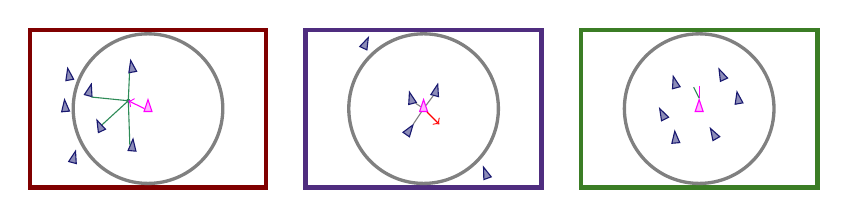
\begin{tikzpicture}
		\onslide<2->{
				\draw[ultra thick, Maroon] (0, 0) rectangle (3, 2);
				\draw[very thick, gray] (1.5, 1) circle [radius=0.95cm];
				%%% Cohesion %%%
				\node[focalfish] (focal2) at (1.5, 1) {};
				\node[fish, rotate=10] (coh1) at ($(focal2) + (-0.2, 0.5)$) {};
				\node[fish, rotate=-15] (coh2) at ($(focal2) + (-0.75, 0.2)$) {};
				\node[fish, rotate=25] (coh3) at ($(focal2) + (-0.6, -0.25)$) {};
				\node[fish, rotate=-5] (coh4) at ($(focal2) + (-0.2, -0.5)$) {};
				\node[fish, rotate=10] (coh5) at ($(focal2) + (-1, 0.4)$) {};
				\node[fish, rotate=5] (coh6) at ($(focal2) + (-1.05, 0)$) {};
				\node[fish, rotate=-15] (coh7) at ($(focal2) + (-0.95, -0.65)$) {};
				
				\draw[SeaGreen] (coh1.south west) -- (1.25, 1.1);
				\draw[SeaGreen] (coh2.south east) -- (1.25, 1.1);
				\draw[SeaGreen] (coh3.north east) -- (1.25, 1.1);
				\draw[SeaGreen] (coh4.north west) -- (1.25, 1.1);
				
				\fill[SeaGreen] (1.25, 1.1) circle [radius=0.75pt];
				
				\draw[Magenta, ->] (focal2.west) -- (1.25, 1.1);}
		\onslide<3->{
				\draw[ultra thick, TarletonPurple] (3.5, 0) rectangle (6.5, 2);
				\draw[very thick, gray] (5, 1) circle [radius=0.95cm];
				%%% Separation %%%
				\node[focalfish] (focal) at (5, 1) {};
				\node[fish, rotate=15] (fish1) at ($(focal) + (-0.15, 0.1)$)  {};
				\node[fish, rotate=-15] (fish2) at ($(focal) + (0.15, 0.2)$) {};
				\node[fish, rotate=-35] (fish3) at ($(focal) + (-0.2, -0.3)$) {};
				\node[fish, rotate=20] (fish4) at ($(focal) + (0.8, -0.85)$) {};
				\node[fish, rotate=-25] (fish5) at ($(focal) + (-0.75, 0.8)$) {};
			
				\draw[thin, gray] (focal) -- (fish1);
				\draw[thin, gray] (focal) -- (fish2);
				\draw[thin, gray] (focal) -- (fish3);
			
				\draw[red, ->] (focal) -- ($(focal) + (0.2, -0.2)$);
		}
		\onslide<4->{
			\draw[ultra thick, OliveGreen] (7, 0) rectangle (10, 2);
				\draw[very thick, gray] (8.5, 1) circle [radius=0.95cm];
				%%% Alignment %%%
				
				\node[focalfish] (focal1) at (8.5, 1) {};
				\node[fish, rotate=15] (align1) at ($(focal1) + (-0.3, 0.3)$) {};
				\node[fish, rotate=25] (align2) at ($(focal1) + (0.3, 0.4)$) {};
				\node[fish, rotate=10] (align3) at ($(focal1) + (0.5, 0.1)$) {};
				\node[fish, rotate=30] (align4) at ($(focal1) + (0.2, -0.35)$) {};
				\node[fish, rotate=5] (align5) at ($(focal1) + (-0.3, -0.4)$) {};
				\node[fish, rotate=27] (align6) at ($(focal1) + (-0.45, -0.1)$) {};
				
				\draw[Magenta] (focal1.north) -- ($(focal1.north) + (0, 0.15)$);
				\draw[SeaGreen] (focal1.north) -- ($(focal1.north) + (-0.07, 0.14)$);
		}
	\end{tikzpicture}
	\begin{equation}
		\onslide<1->{
		F_{i_N} = \sum\limits_{j=1}^{N}\bigg(}
		\onslide<2->{ W_{a}\big( \textcolor{Maroon}{C_{a} \frac{p_{j} - p_{i}}{d^{2}} } }
		\onslide<3->{\textcolor{TarletonPurple}{- C_{r}\frac{p_{j} - p_{i}}{d^{4}}} \big)}
		\onslide<4->{ + W_{d} \big(\textcolor{OliveGreen}{\frac{v_{j}}{||p_{i} - p_{j}||} \big) \bigg) } }
	\end{equation}
\end{frame}

\begin{frame}
	\frametitle{Simulations}
%	\movie{}{images/2048fish-quicktime.mov}
\end{frame}


\end{document}